\documentclass[12pt]{article}
\usepackage[margin=1in, paperwidth=8.5in, paperheight=11in]{geometry}
\usepackage{amsfonts}
\usepackage{graphicx}
\usepackage{enumitem}
\usepackage{setspace}
\usepackage{url}


\newcommand{\HRule}{\rule{\linewidth}{0.5mm}}
\newcommand{\prob}{\textsf{Pr}}

\begin{document}
%%%%%%%%%%%%%%%%%%%%%%%%%%%%%%%%%%%%%%%%%%%%%%%%%%%%%%%%%%%%%%%%%%%%%%%%%%%%
\begin{titlepage}
\begin{center}
\topskip0pt
\vspace*{\fill}
%\includegraphics[width=0.15\textwidth]{logo.png}~\\[1cm]
\textsc{\Large 36-350 Statistical Computing}\\[8pt]
\textsc{\Large Final Project}\\[0.5cm]

\HRule \\[0.4cm]
{\LARGE \bfseries Markov Chain Genetic Models \\[0.4cm]}
{\normalsize \bfseries Simulating the DNA of \textit{Dictyostelium discoideum}\\[0.4cm]}
\HRule \\[1.5cm]

\begin{minipage}{0.4\textwidth}
\begin{flushleft} \normalsize
\emph{Author:}\\
Kairavi \textsc{Chahal}
\end{flushleft}
\end{minipage}
\begin{minipage}{0.4\textwidth}
\begin{flushright} \normalsize
\emph{Group Members:} \\
Tony \textsc{Yang}\\
Julian \textsc{Zhou}
\end{flushright}
\end{minipage}
\\[4cm]
{\normalsize \today}
\vspace*{\fill}
\end{center}
\end{titlepage}
%%%%%%%%%%%%%%%%%%%%%%%%%%%%%%%%%%%%%%%%%%%%%%%%%%%%%%%%%%%%%%%%%%%%%%%%%%%%
\onehalfspacing
\section{Introduction}
This project uses Markov chains to model the chromosomes of the soil-living slime mould \textit{Dictyostelium discoideum}. Using this model, chromosomes are simulated and compared to the originals to test how well the model fits the data.
\subsection{Markov Chains}
Markov chains are used to model random processes and subsequently simulate the same process to create data that is usually used to test another algorithm or model.\footnote{\url{http://en.wikipedia.org/wiki/Markov_chains}} Markov chains are usually said to be `memoryless,' i.e., they do not depend on prior information. However this is misleading, as they use certain information from a prior sequence. The length of this prior sequence determines the order of the Markov chain, usually denoted by \textit{k}.
\\[8pt]
A Markov chain models the data by looking at each step in a process and determining the probability of that step being in a certain state, given the previous \textit{k} steps. This model also postulates that the \textit{i}th step is independent of any steps before the (\textit{i-k})th step. Mathematically, Markov chains can be represented as:
$$
\prob(X_i = x | X_{1} = x_1, ..., X_{i-1} = x_{i-1}) = \prob(X_i = x | X_{i-k} = x_{i-k}, ..., X_{i-1} = x_{i-1})
$$
Empirically, Markov models are created by analysing data and determining the proportions of each state, given the previous \textit{k} steps were in a certain state. This yields a Markov matrix, which contains the probabilities of each state happening given the previous states. Simulations are then created by sampling the possible states using the probabilities from the Markov matrix.
\subsection{Data}
For this project, the data was the genome of the \textit{Dictyostelium discoideum} organism. The genome consisted of 11 chromosomes, which in turn are made up of four possible bases: A, C, G and T. The length of the chromosomes ranged between 16,660 bases (Chromosome 3F) and 8,484,197 bases (Chromosome 2). Markov chains were used to model the sequences of bases. In the context of the data, the Markov chain determined the probability of the \textit{i}th base being A, C, G or T, given the previous \textit{k} bases in that chromosome.
\subsection{Objective}
The main aim of this project was to write code that could model the chromosomes and subsequently simulate `fake' chromosomes from the Markov matrices and then compare the the original and simulated chromosomes, using R. The comparison was then used to answer two questions of interest:
\begin{enumerate}
\item How does the order of the Markov chain affect the fidelity of the simulations?
\item How are simulations different for different chromosomes, particularly chroomosomes of different lengths?
\end{enumerate}
A successful solution to this objectives of this project would include R code that is easy to understand and run and the results of which should either answer the questions of interest or be able to be analysed to answer the questions of interest.
\section{Approach and Solution}
The approach to achieving the objective of this project was broken into four steps, as shown in Figure \ref{fig:algorithm}.
\begin{figure}
  \centering
  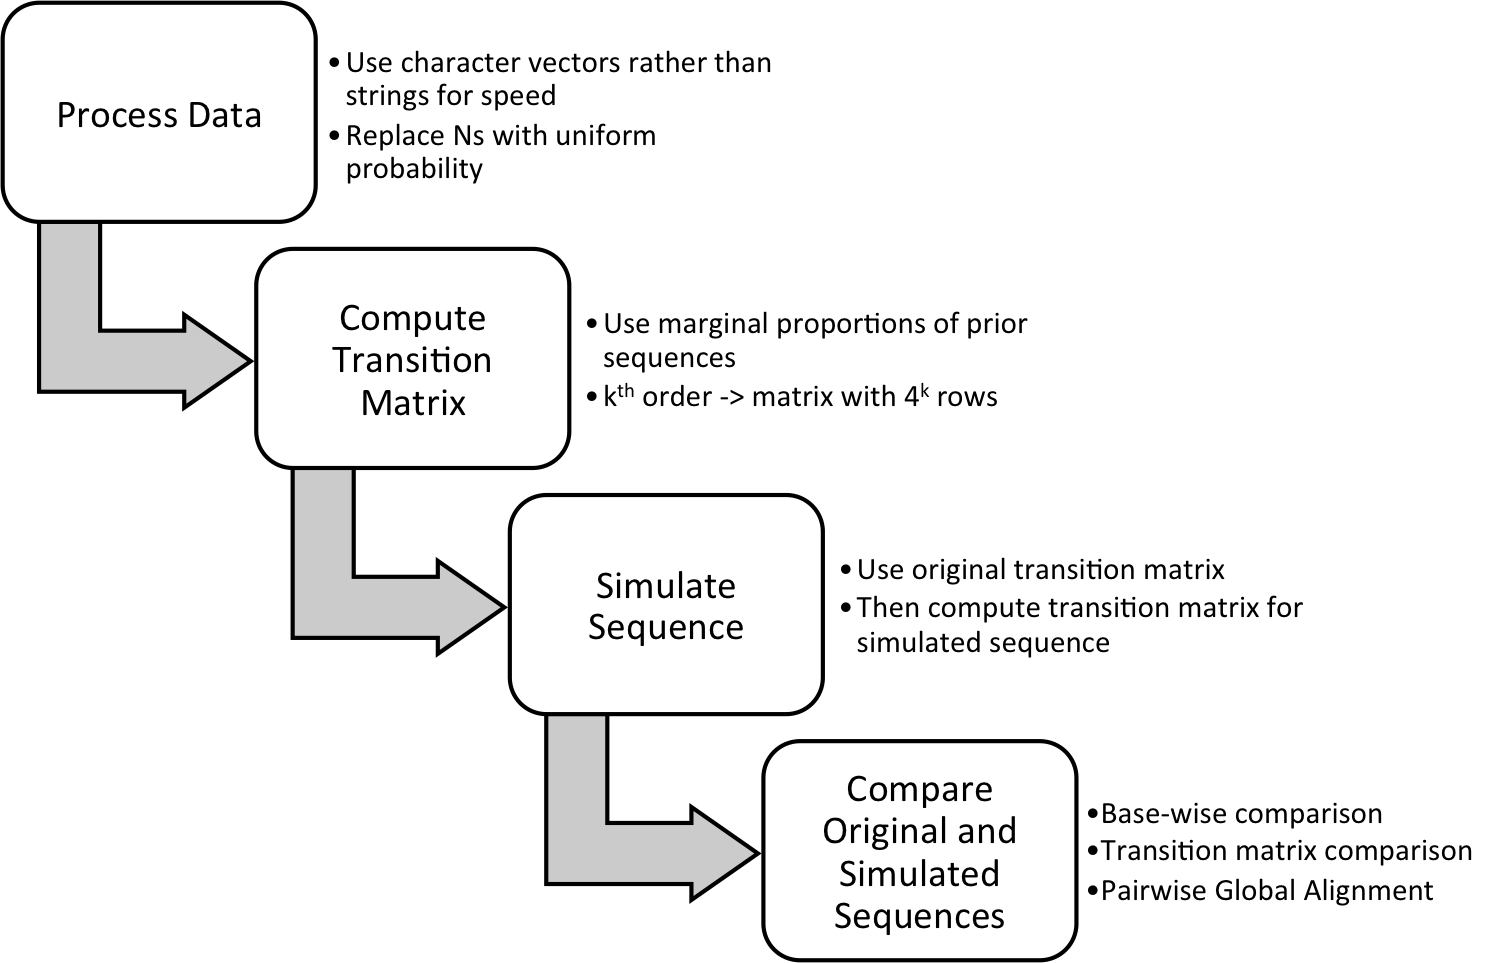
\includegraphics[scale=0.5]{algorithm.png}
  \caption{Overall Approach to the Project\label{fig:algorithm}}
\end{figure}
\subsection{Process Data}
The data was originally formatted in FASTA format,\footnote{\url{http://en.wikipedia.org/wiki/FASTA_format}} which is a commonly used format for storing data about chromosomes. R already contains a package \texttt{seqinr}\footnote{\url{http://cran.r-project.org/web/packages/seqinr/index.html}} that can read a text file containing chromosome sequences and return a vector of characters in R, where each character represents a base in the chromosome.\footnote{After running simulations and realizing how time consuming they are, we decided it might be more efficient to convert these character vectors into integer vectors. We tested this on vectors of various lengths and concluded that using integers is indeed faster than using characters, and that improvement in speed is more noticeable for longer vectors. However, we were unable to implement this method in our code. This remains for future iterations of this project.}
\\[6pt]
Another challenge in reading in the data was that parts of the chromosomes contained Ns, which is a symbol for undetermined bases. This resulted in incomplete data and there were three ways to deal with this missingness:
\begin{enumerate}
\item The simplest strategy was to completely drop all the Ns from the data and then proceed as normal. However, this is the least ideal way to approach this, since it would have the greatest impact on the results produced.
\item The solution implemented was to simply replace the Ns with either A, C, G or T, with a uniform probability of 0.25. While this does not entirely ensure the results will be unbiased, it does not get rid of any data, and over the course of several simulations, the randomness will be balanced.
\item The most difficult to implement solution would be to replace the Ns using probabilities from the chromosome prior to the Ns. However, many Ns were at the beginning of the chromosome, with no prior sequence to condition on.
\end{enumerate}
\subsection{Compute Markov Matrix}
Computing the Markov matrix was the toughest algorithm to implement, as it required a lot of data-structure manipulation. The basic algorithm used in computing the Markov matrix was this:
\begin{enumerate}
\item Determine all subsequences of length \textit{k}+1 of the given chromosome. For example, if the chromosome was \texttt{"ACGTAGCT"} and the order was 2, the subsequences would be \texttt{"AC"}, \texttt{"CG"}, \texttt{"GT"}, \texttt{"TA"}, \texttt{"AG"}, \texttt{"GC"} and \texttt{"CT"}.
\item Determine the counts of each subsequence, and then group the subsequences by the last base, resulting in four groups. Each of these groups makes up one column of the Markov matrix.
\item Each row is then determined by counting the occurrences of the prior sequence. Each element in a row is then divided by the sum of that row to determine the probability of that particular subsequence occuring. Any subsequences that do not appear in the chromosome are filled in with a probability of 0.25.
\end{enumerate}
\subsection{Simulate Chromosomes}
Simulating the chromosome was the most time-consuming process, but fairly easy to implement. An important decision to be made was what the first \textit{k} bases in the simulated chromosome would be. The two options were to either randomly sample a sequence of length \textit{k} with uniform probability or to use the first \textit{k} bases from the original chromosome.\footnote{Although we went with the latter option, I think it would be interesting to see how well the simulated chromosomes match the original chromosomes when they start with a completely random `seed' prior sequence.} The algorithm used was:
\begin{enumerate}
\item Get an initial prior sequence and generate the next base by selecting the row containing the prior sequence from the Markov matrix.
\item Update the simulated sequence to include the new base and move the prior sequence selection window one base to the right.
\item Continue this process until a simulated sequence the same length as the original sequence is generated.
\end{enumerate}
\subsection{Compare Original and Simulated Chromosomes}
Three standards were used to compare the original chromosomes and the simulated chromsomes:
\begin{description}
\item[Base-wise Comparison] This method compares each base in the simulated chromosome to the corresponding base in the original chromosome. The final result of this comparison is a list of the number of absolute matches as well as individual proportions of each base matched, i.e., proportion of As matched, etc.
\item[Markov Matrix Comparison] This method calculates the Markov matrix of the simulated chromosome and returns a statistic $\theta$ that determines how close the two are.
$$
\theta = \frac{\sum |M_{orig} - M_{sim}|}{4 \times 4^k}
$$
\item[Pairwise Global Alignment] This comparison is implemented using the R package \texttt{biostrings}.\footnote{\url{http://www.bioconductor.org/packages/2.14/bioc/html/Biostrings.html}} It assigns each comparison a score based on the number of matches, mismatches and gaps, by rewarding and penalizing each type of match.
\end{description}
\section{Simulation and Analysis}
Each chromosome was simulated 10 times, with Markov chain order of 1, 2 and 3. However, the longer chromosomes (Chromosomes 1, 2, 3, 4, 5 and 6) were unable to finish simulations due to time constraints. However, five chromosomes were successfully simulated 30 times each - 10 times per \textit{k} = 1, 2, and 3. The data collected from running these simulations produced the charts in Figures \ref{fig:basewise}, \ref{fig:theta} and \ref{fig:pairwise}. The two questions of interest are then answered as follows:
\begin{description}
\item[How does the order of the Markov chain affect the simulations?] The Pairwise Global Alignment scores seem to decrease as \textit{k} increases, as do the differences between the original and simulated Markov matrices. This suggests that a higher-order Markov chain produces simulated chromosomes that are more varied from the originals.
\item[How are simulations different for different chromosomes?] Length of the chromosome appears to be a significant factor in determining how well the original and simulated chromosomes match.
\end{description}
\begin{figure}
  \centering
  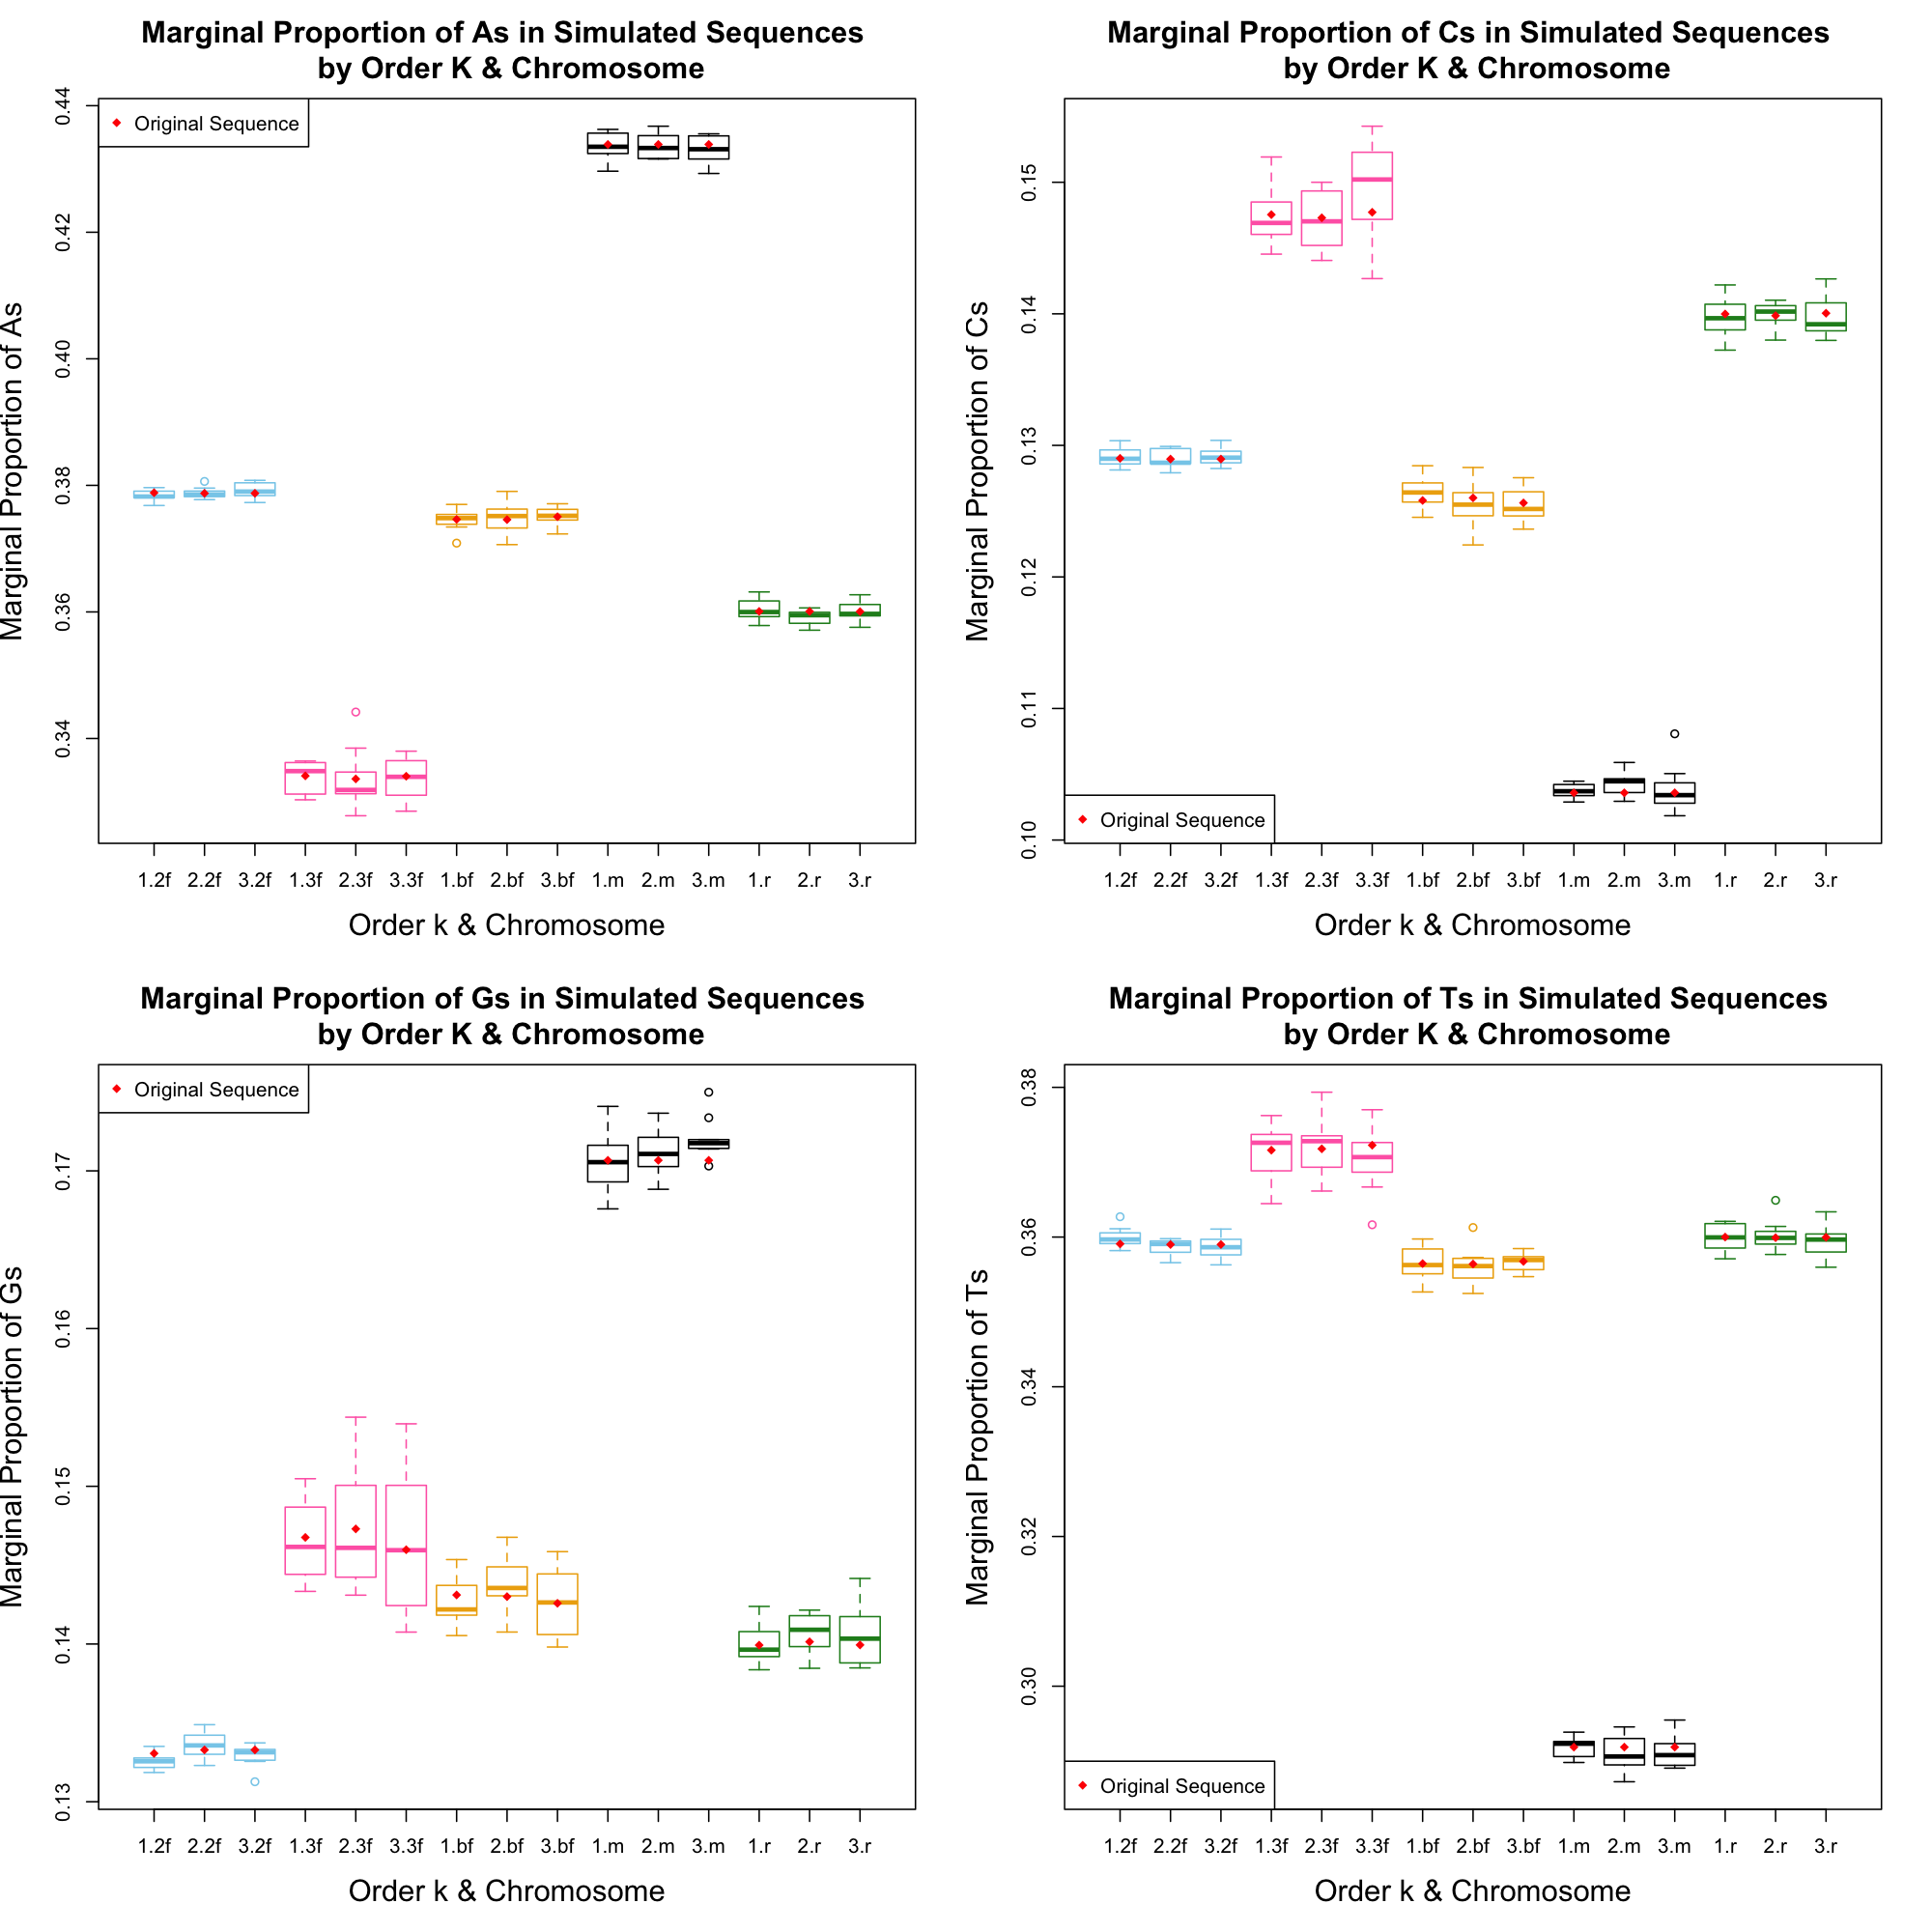
\includegraphics[scale=0.2]{basewise.png}
  \caption{Proportion of Bases vs. Chromosome and Order\label{fig:basewise}}
\end{figure}
\begin{figure}
  \centering
  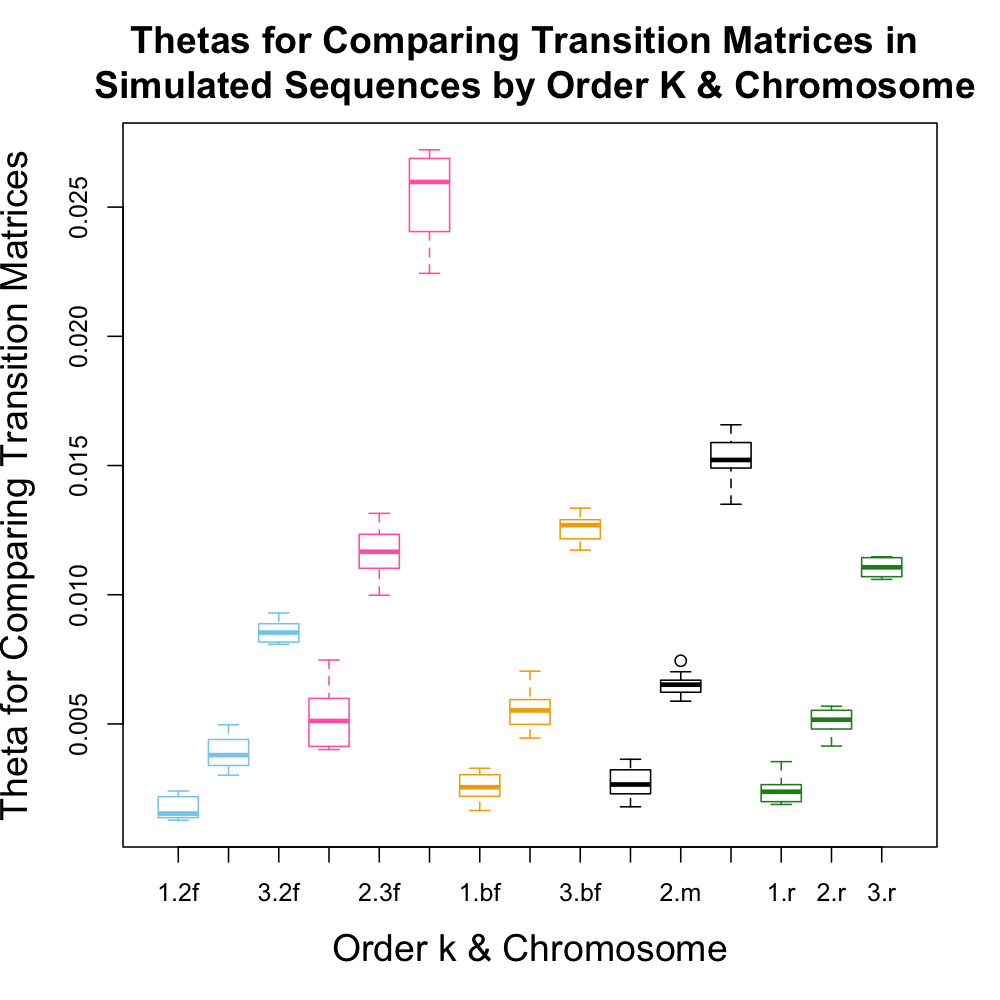
\includegraphics[scale=0.25]{theta.png}
  \caption{Theta vs. Chromosome and Order\label{fig:theta}}
\end{figure}
\begin{figure}
  \centering
  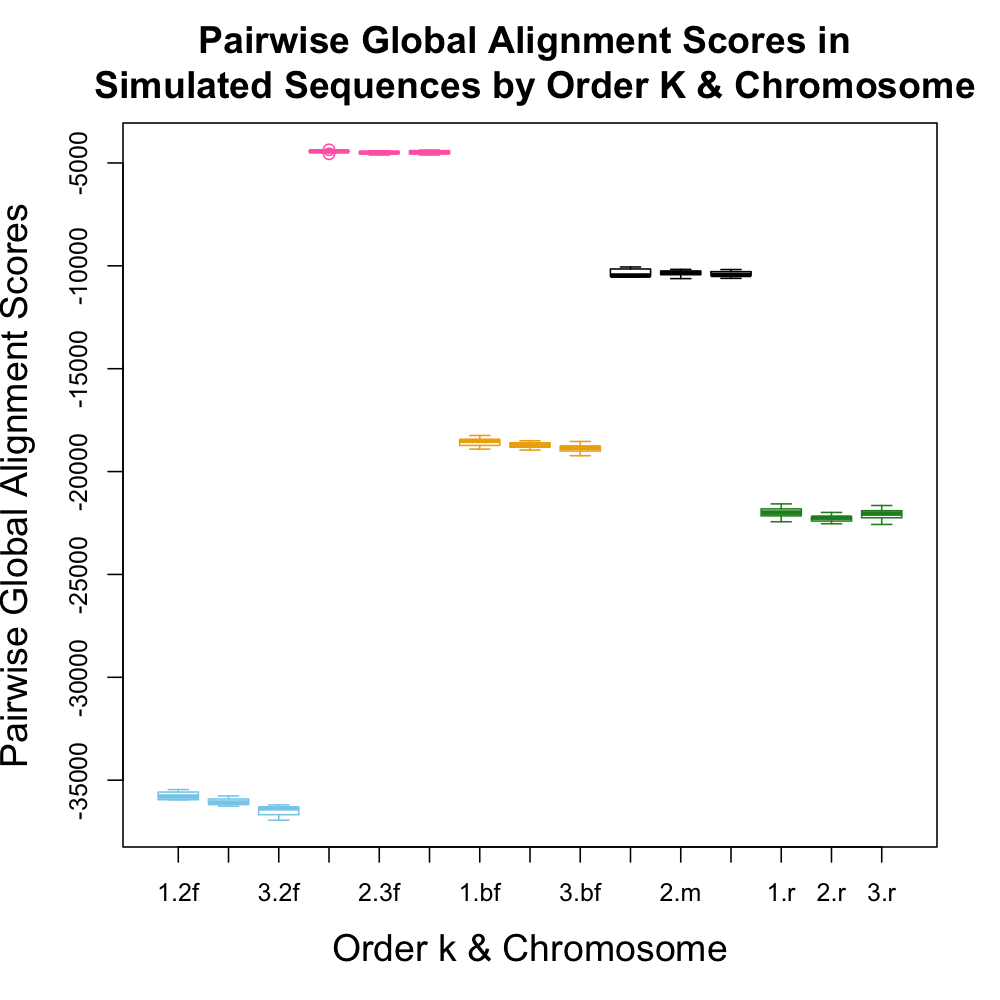
\includegraphics[scale=0.25]{pairwise.png}
  \caption{Pairwise Global Alignment Score vs. Chromosome and Order\label{fig:pairwise}}
\end{figure}

\end{document}